\documentclass{article}
\usepackage[utf8]{inputenc}
\usepackage{tikz}
\usepackage{amsmath}
\usepackage{algpseudocode}

\newcommand{\grid}[0]{
        \draw[step=1cm,color=gray] (0,0) grid (5,5);
        
        \foreach \y in {0.5,1.5,2.5,3.5,4.5}
          \foreach \x in {0.5,4.5}
            \node at (\x,\y) {1};
        
        \foreach \y in {0.5,4.5}
            \foreach \x in {1.5,2.5,3.5}
              \node at (\x,\y) {1};
        \node at (2.5,2.5) {\textsf{P}};
}


\title{Raycster with SDL and C++}
\author{Sam Laister}
\date{November 2022}

\begin{document}

\maketitle

\section{Introduction}
Hello, Welcome to my writeup on a recent passion, a raycaster! I've been interested in 
DOOM's (1996) renderer for some time now. However jumping that far into the deep end 
isn't my style. So let's start with it's predecessor, Wolfenstein 3D (1992). 

They say that the best way to learn is to teach. So I'm going to try and teach you, 
providing code snippets from my own program. The source code can be found on my
github page\footnote{https://github.com/Soup666/SDL-Raycaster\_v1}

\section{The Basics}
I want to split this writeup into 3 sections, the maths, translating that to code, and 
finally the SDL implementation. Lets start with the basics of the Maths involved.

Say you have a x and y coord representing a player, the goal is to shoot rays from left 
to right and then draw vertical pixels depending on how far the ray has travelled. But this
arises questions such as how do we calculate if a ray has hit a wall? How do we know how 
far the ray has travelled? How do we know what direction to shoot the ray? etc. I'm going to
present a simplified situation and break it down.

\subsection{Setting the Scene}
Imagine you have a simple 2D grid, lets say 5 by 5. The player is in the middle of the grid, 
so (2.5, 2.5). In said grid, a 1 represents a wall, and a 0 represents an empty space. As 
demonstrated below.

\begin{center}
    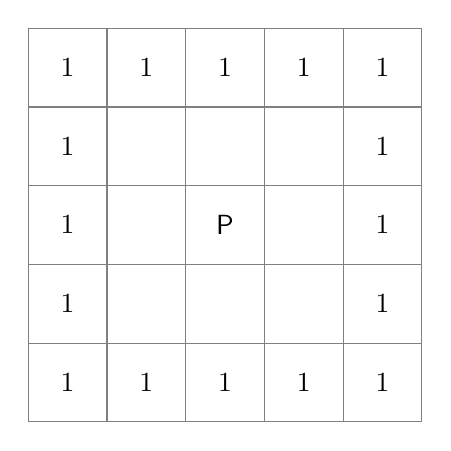
\begin{tikzpicture}
    \grid{}
    \end{tikzpicture}
\end{center}

The way we're going to create a raycaster, is by shooting different rays for horizontal and
vertical walls, then drawing the smallest ray as either a vertical wall or horizontal wall,
respectfully. The way we define a vertical wall or horizontal wall is simple. Take a 1 from
the above diagram, A vertical wall is a wall that is either to the left or right and spans 
the length of the unit. A horizontal wall is obviously a wall that is either above or below.
Wall's in this raycaster don't have a normal variable to take into account.

For this example, we're going to set the player's direction to +59.04 $\deg$, so facing north east.
And we'll shoot a single ray the same direction. 

\subsection{Horizontal Ray}

\begin{center}
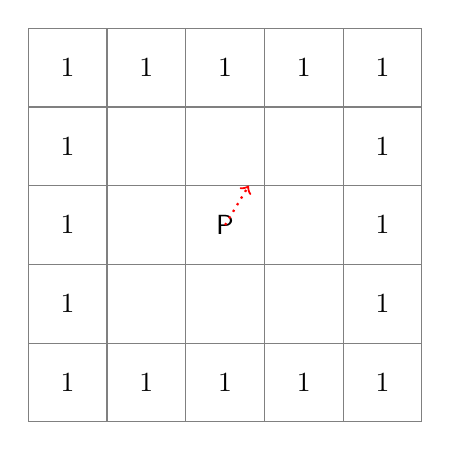
\begin{tikzpicture}
    \grid{}
    \draw[red, thick, dotted, ->] (2.5,2.5) -- (2.8, 3);
    \end{tikzpicture}
\end{center}

Okay lets get into some maths. We want to calculate the nearest wall from the players position,
(2.5,2.5). In pixel position, this would be (250,250). Assuming 0,0 is top left, and we're 
looking east, we can the nearest horizontal boundary. We know:

\begin{equation}
    \begin{split}
        & pa = 59^\circ  (1.031rad) \\
        & px = 250 \\
        & py = 250 \\
    \end{split}
\end{equation}

We can then calculate the ray's first x and y.
\begin{equation}
\begin{split}
    & unitW = 500 / 5 = 100 pixels \\
    & ry = floor (playerY / unitW ) * unitW - 0.001 \\
    & rx = playerY * \frac{1}{\tan 1.031} + playerY \\
\end{split}
\end{equation}

NOTE the -0.001 is to slightly push it in the bounds of the next square, so we don't check the 
current players square. We only do this if the player is looking in the negative y direction.

Giving us $(279.96, 200)$. Great! However we can do better. A grid is made up of squares, so what if
we calculated an offset as well to repeat the proccess. Let me give you an example.

We introduce $ox$ and $oy$. As per,

\begin{equation}
    \begin{split}
        & yo = -100 \\
        & xo = -yo * \frac{1}{\tan 1.031} \\
    \end{split}
\end{equation}

Giving us $yo = -100$ and $xo = 38.346$. Let's demonstrate this on a graph.

\begin{center}
    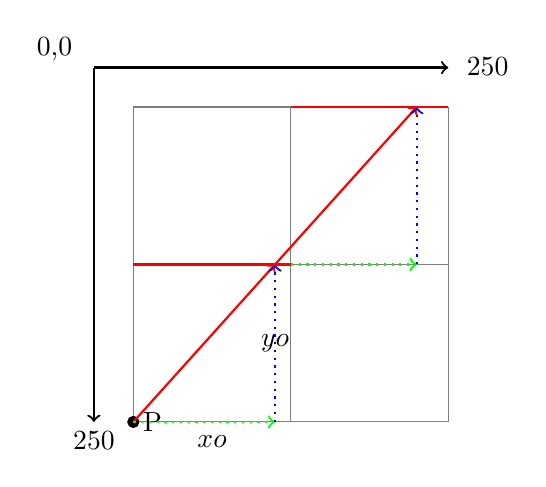
\begin{tikzpicture}
    \draw[step=2cm,color=gray] (0,0) grid (4,4);
    \draw[black, thick, ->] (-0.5,4.5) -- (-0.5,0);
    \draw[black, thick, ->] (-0.5,4.5) -- (4,4.5);
    \draw (-0.5, 0) node[below] {250};
    \draw (4.5, 4.75) node[below] {250};
    \draw (-1, 5) node[below] {0,0};

    \filldraw[black] (0,0) circle (2pt) node[anchor=west]{P};

    \draw[red, thick, ->] (0,0) -- (1.8, 2);
    \draw[green, thick, dotted, ->] (0,0) -- (1.8, 0);
    \draw[blue, thick, dotted, ->] (1.8,0) -- (1.8,2);
    
    \draw[red, thick, ->] (1.8,2) -- (3.6, 4);
    \draw[green, thick, dotted, ->] (2,2) -- (3.6, 2);
    \draw[blue, thick, dotted, ->] (3.6,2) -- (3.6, 4);

    \draw[red, thick] (0,2) -- (2,2);
    \draw[red, thick] (2,4) -- (4,4);

    \draw (1, -0.25) node {$xo$};
    \draw (1.8, 1) node {$yo$};
    \end{tikzpicture}
\end{center}

Here, you can see we intersect two horizontal lines. Perfect. We'll eventually be checking 
if the square north of the intersection is a wall, and if it is we return the ray length.

\subsection{Multidirectional Rays}

Ok, so so far we have a working algorithm for calculating the angle of a ray based off the
players current rotation! Great, as long as the player is looking north east. The formulae changes
slightly depending on the angle of the player. For example, we substracted -0.001 so the ray landed 
within the box, however if the player is looking 180 $\deg$ that no longer functions as intended.

To solve this, we can set bounds for different behaviours. We'll start by assigning a $rayangle$ variable

\begin{center}
    $ra = pa + offset$
\end{center}

We can decide which direction the player is looking by applying $\cos$ or $\sin$ to this variable.

\begin{center}
\begin{algorithmic}
    \State $ra \gets pa$
    \If{$\cos ra\geq 0.001$} 
        \State \dots
        \State // Looking left
    \EndIf 
    \If{$\cos ra\leq -0.001$}
        \State \dots
        \State // Looking right
    \EndIf 
    \State $ra \gets pa$
    \If{$\sin ra\geq 0.001$} 
        \State \dots
        \State // Looking Up
    \EndIf 
    \If{$\sin ra\leq -0.001$}
        \State \dots
        \State // Looking Down
    \EndIf 
    \end{algorithmic}
\end{center}

\end{document}
